\section{Problem Model}\label{sec_extrafunc}
The software allocation problem is a type of job shop scheduling with constraints, as such it is a discrete optimization problem \cite{}. The solution to the allocation problem is represented by a vectormatrix $\x=\{\xsp{k}:k=1,...,N_a\}$, where \ttxsp{k} is a matrix of size $N_c\times K$, and \ttssx{x}{k}{ij}$=k\in \{1,…,N_m\}$ represents the mapping of the software component replica \ttssx{c}{k}{ij} to the computation node $m_k$.
\begin{equation}
\label{fig_pso_solution_representation}
\bspx{k}=
\begin{bmatrix} 
\ssx{k}{11} & \ssx{k}{12} & \dots & \ssx{k}{1K}\\
\ssx{k}{21} & \ssx{k}{22} & \dots & \ssx{k}{2K}\\
\vdots & \vdots & \ddots & \vdots\\
\ssx{k}{N_c1} & \ssx{k}{N_c2} & \cdots & \ssx{k}{N_cK}
\end{bmatrix}
\end{equation}

In this work, the main objective of the allocation problem is to satisfy the user-defined requirements, namely reliability requirements, end-to-end timing requirements, and criticality of the software applications $A_i$ by effectively mapping the software components to the computation nodes, $C^{(k)}\mapsto M$. Furthermore, the components are allocated efficiently to minimize the total power consumption $Power(\textbf{x})=\sum_{m\in M'}{P_{m}(\textbf{x})}$ of the applications by selecting lower-power consuming nodes $M'\subseteq M$, provided the requirements are met, where $P_{m}(\textbf{x})$ is the power consumption of node $m$ on the mapping $\textbf{x}$. Power consumption, in this context, refers to the energy usage of electronic components in the integrated circuits of the node, e.g., processor, memory, I/O devices, etc., per time unit. 

%Power consumption refers to the energy usage of electronic components in an integrated circuit, e.g., processor, memory, I/O devices, etc., per time unit. 
There are several power consumption models and different techniques to estimate the power consumption of a computing node. In this work, we employ a technique based on processor load (or \textit{Processor Utilization}) to estimate the average power consumption of a computation node. Specifically, we use the linear polynomial model proposed by Fan et al. \cite{Fan2007PowerComputer}, which is shown in (\ref{eqn_powerconsumption}). The model states that the power consumption of a node is directly proportional to its load, and is inductively formulated from experimental results:
\begin{equation}
\label{eqn_powerconsumption}
f_p(u)=P_{idle} + (P_{busy}-P_{idle})*u,
\end{equation}

where $u$ is the utilization (or load) of a computation node, $p_{idle}$ and $p_{busy}$, respectively, refer to the power consumption of a node measured at minimum and maximum processor loads. Such measurements can be obtained by running performance benchmark suits, e.g., MiBench \cite{Guthaus2001MiBench:Suite}, AutoBench \cite{EMBC2018AutoBenchProcessors}, etc., which is computed based on the utilization of the node via the linear power consumption model shown in Equation (\ref{eqn_powerconsumption}).

Consequently, the power consumption of a node $m$ for a given mapping $\textbf{x}$ is computed using Equations (\ref{eqn_powerconsumption_x}-\ref{eqn_util_component}), by calculating first the node's utilization $U_m(\textbf{x})$ using Equation (\ref{eqn_util_x}). The node's utilization is computed from the set of components allocated to it (which are $\forall_{ij} x_{ij}=m$) using Equation (\ref{eqn_util_x}). And the utilization of a component on the node $m$ is computed from its constituent tasks $T_c$ using Equation (\ref{eqn_util_component}).
\begin{align}
	\label{eqn_powerconsumption_x}
nodPow(\textbf{x}) & =f_p(nodUti(\textbf{x},m))                         &  \\
	\label{eqn_util_x}
nodUtil(\textbf{x},m)           & = \sum_{k}{\sum_{i}{\sum_{j}{comUtil(m,c)}}}|\xkij=m         & \text{, where } c=\sss{C}\\
	\label{eqn_util_component}
comUtil(m,c)              & = \sum_{r\in c.R} \frac{r.e_m}{r.\tau.P}, &
\end{align}

where $c.R$ is set of runnables in component $c$, $r.e_m$ and $r.\tau.P$ are the execution of runnable $r$ on node $m$ and its period, respectively.

The applications requirements are modeled as constraints that need to be satisfied in the allocation problem. The constraints formulations are shown in the following subsections, respectively for reliability, timing and other design constraints such as related to runnables-to-tasks merging and replication.

\subsection{Software Application Reliability Constraints}\label{subsec_reliability_constraint}
The applications reliability constraints ensure the mapping $\textbf{x}$ satisfies the user-defined reliability requirements, that is $ \forall k\in [1,n_A]\ \rel_{A_k}(\xsp{k})\leq RelReq_{A_k}$. 
The reliability  is computed from the execution framework that is provided to run the application, which consists of computation nodes \ttssp{M} and the shared CAN bus B, as shown in Equation (\ref{eqn_appreliability_app}). The nodes \ttssp{M} host the components \ttssp{C} and are determined by searching the mapping \ttxsp{k}  in polynomial time using Equation (\ref{eqn_nodes_app}).
\begin{align}
	\label{eqn_appreliability_app}
	&Reliability_{A_i}(\x)=Reliability_{A_i}(\ssp{M})*Reliability(B)\\
	\label{eqn_nodes_app}
	&\ssp{M}=\{e|e\in M \land \forall ij (e=m_h) \},\mbox{ where } h=\ssx{k}{ij} 
\end{align}

The reliability of the nodes, $Reliability_{A_i}(\ssp{M})$ with respect to the application ${A_k}$ is calculated using the \textit{state-enumeration} technique \cite{Lucet1999ExactReliability}  as shown in Equations (\ref{eqn_appreliability}). According to the technique, the reliability is basically the total probability that the application $A_k$ \textit{functions} under mutually exclusive and uniformly distributed failure-events of the nodes, represented by $\ssp{\mathcal{F}}(\ssp{M})=\{\textbf{0},\textbf{1}\}^{\ssp{M}}$, where  \textbf{0} means node fails, \textbf{1} means  node is operational. An event $\omega\in \mathcal{F}_{A_k}(\ssp{M})$ represents the states of nodes by a sequence of 0-1 variables $(b_1,...,b_n)$, where $\omega.b_i$ denote the state of node $m_i\in \ssp{M}$. %as the state of the nodes $\ssp{M}=\{e_1,...,e_n\}$ by $s\in \ssp{\mathcal{F}}(\ssp{M})=(b_{e_1},...,b_{e_n})$, where $n=|\ssp{M}|$, whereas the state of a node is referenced by $s.b_{e}$.
\begin{align}
\label{eqn_appreliability}
Reliability_{A_i}(\ssp{M})&=\sum_{s\in \ssp{\mathcal{F}}|g(A_i, s)=1}probability(s)
\end{align}

The fact that an application functions $g(A_k, s)$ is defined via its inverse, which is \textit{software application failure}, deductively as follows:
\begin{definition}[Software Application Failure]
The application $A_k$ fails in the event $\omega \in \ssp{\mathcal{F}}(\ssp{M})$ if there exists a component type \ttsss{c} where all of its replica \ttsss{Q} \textit{fail}, otherwise, the application functions, as shown in Equation (\ref{eqn_app_failure}).  A component replica $\sss{q}[k][ij]\in \sss{Q}$ fails if the node that host it $m_h$ fails, where $h=\xkij$.  
\begin{align}
\label{eqn_app_failure}
g(a, \omega)&= 
\begin{cases}
\textbf{0} & \mbox{ if } \exists i\forall j\ (m_h\in \sss{M}[k][\omega] )\\
\textbf{1} & \mbox{ otherwise }
\end{cases}\\
\label{eqn_appreliability_node_s}
\sss{M}[A_k][\omega]&=\{e|e\in \ssp{M} \land (\omega.b_e=1) \},
\end{align}
\end{definition}
where \ttsss{M}[k][\omega] denote the nodes that function at the event $\omega$, and can be found by searching the nodes \ttssp{M} with state $\omega.b_e=1$ in constant time , as show in Equation (\ref{eqn_pro}).

The probability that a nodes-failure event $\omega$ occurs is computed as a product of the probabilities of its consitutuent elements $\omega.b$ as shown in Equation (\ref{label}).
\begin{equation}
\label{eqn_pro}
	\prod_{(m,b)\in (M,\omega)}{\lambda_m*(1-b)+(1-\lambda_m)*b}
\end{equation}
where $\lambda_m$ is the failure-rate of node $m$.

\subsection{Timing constraints}
The timing constraints ensure that the applications are schedulable on the execution platform, that is the tasks and cause-effect chains of each application meet their deadlines. The schedulability of each task is checked using the worst-case response-time anlaysis presented in \ref{subsec_responsetimeanalysis}, and the schedulability of cause-effect chains is checked using the delay analysis shown in Subsection \ref{subsec_causeeffectchains}. To calculate the delay, the response time of tasks is a prerequisite, therefore, the latter is calculated first as follows.

\subsection{Tasks Timing constraints}
For a mapping \x, the worst-case response time of the tasks in the distributed system \ttsss{T}[k][i,j] should be less than or equal to their respective deadlines, that is $\forall k\forall ij\ ResponseTime_\tau(\x)\leq Deadline_\tau$, where $\tau \in$ \ttsss{T}[k][i,j]. To calculate the response time of each task, first we drive the set of components and tasks mapped to each node in the system, respectively using Equation (\ref{eqn_components_nodes}) and (\ref{eqn_tasks_nodes}), all in polynomial time. In the former, we search the mapping \ttx and collect components \ttsss{q}[k][i,j] mapped to each node $m_h$. In the latter, we infer the tasks mapped to each component by invoking the mapping function $\zeta(\sss{q}[k][i,j])$.
\begin{align}
\label{eqn_components_nodes}
Q_{m_h}&=\left\{e | \forall k\forall ij\ (\xkij = h \land e\in \sss{Q}\right\}& \mbox{ for all } h=1,...,n_M\\
\label{eqn_tasks_nodes}
T_{m_h}&=\{e | \forall q\in Q_{m_h} \ \zeta(q) \}& \mbox{ for all } h=1,...,n_M
\end{align}

Then, we calculate the response time of each task $\tau \in T_{m_h}$ by invoking the response-time analyais formula and construct the tasks timing constraints as shown in Equation (\ref{eqn_tasks_constraints}).
\begin{align}
\label{eqn_tasks_constraints}
\forall \tau\in T_{m_h} RT(\tau,m_h)&\leq Deadline(\tau)& \mbox{ for all } h=1,...,\n{M}\\
\end{align}

\subsection{Cause-effect Chains Timing constraints}
For a mapping \x, the delay of cause-effect chains in the system should be less than or equal to their respective deadlines, that is $\forall k\forall ij\ Delay_\gamma(\x)\leq E2eReq_\gamma$. In this work, we assume a particular type of end-to-end delay, known as age delay, which is discussed in Subsection \ref{subsec_causeeffectchains}. 

In order to calculate, the cause-effect chain delays, the messages for a mapping \x should be identified first using Equation x. Then we update the cause-effect chains that communicate over the shared CAN bus to incorporate the messages in the chains using Eqaution x. We assume each task communicating over the network, uses a message with the same priority and period that of the predecessor task.

\begin{figure}
	\centering
	\includegraphics[width=0.5\linewidth]{img/cause_effect_chain_ntk}
	\caption[A cause-effect chain deployed on node 1 and node2.]{}
	\label{fig:causeeffectchainntk}
\end{figure}


For a multirate cause-effect chain   timing constraints on the cause-effect chains of the applications
The software application can be considered as a set of cause-effect chains, which are directed paths in the application graph, e.g.,  activation of a cruise control system by pressing a rotary-wheel on the dashboard, slowing down of a car by pressing the brake pedal, etc. Each cause-effect chain is annotated with an end-to-end timing requirement that specifies the maximum time between a stimulus and the corresponding response of a chain. A cause-effect chain can be hosted on a single node or multiple nodes as illustrated in Figure \ref{fig_datachainsingle} and Figure \ref{fig_datachainmulti}, respectively. Moreover, it can be activated by a single activation pattern, or multiple activation patterns (multirate).
\begin{figure*}[h!]
    \centering
    \begin{subfigure}[b]{0.25\textwidth}
    \includegraphics[trim=0 0 0 0,clip,width=\textwidth]{datachain_singlenode}
    \caption{Deployment on a Single Node.}
    \label{fig_datachainsingle}
    \end{subfigure}
    ~ %\quad, \qquad, \hfill 
    \begin{subfigure}[b]{0.365\textwidth}
    \includegraphics[trim=0 0 0 0,clip,width=\textwidth]{datachain_multinode}
    \caption{Deployment on Multiple Nodes.}
    \label{fig_datachainmulti}
    \end{subfigure}
   ~\vspace{-0.2cm}
    \begin{subfigure}[b]{0.35\textwidth}
    \includegraphics[width=\textwidth]{timedpath}
    \caption{Timed Paths of Age and Reaction Delays.}
    \label{fig_timedpath}
    \end{subfigure}
    \caption{Cause-effect Chain with Three Activation Patterns.}
    \label{fig:datachain}
\end{figure*}

The calculation of data-propagation delays in multirate software applications is not trivial due to the oversampling and undersampling effects, caused by the different activation patterns. Consequently, there are different delay semantics, which differ depending on the timed paths through which the data is propagated from the input to the output of the chains~\cite{mubeen2013support}. In this work, we focus on the \textit{age} and \textit{reaction} delays, which are the most widely used delay semantics in the automotive embedded systems. The two delays in a cause-effect chain that is distributed over two nodes  are demonstrated in Figure~\ref{fig_timedpath}. The tasks t1 and t2 execute on one node, whereas task t3 executes on the second node. Note that t2 communicates with t3 via a network message, that is not shown in the figure for simplicity. The red inverted arrows in Figure~\ref{fig_timedpath} represent the arrival of events at the input of the chain, whereas the dashed-curve arrows represent the timed paths through which the data propagates from the input to the output of the chain. The age delay is the time elapsed between a stimulus and its corresponding latest non-overwritten response, i.e., between the $2^{nd}$ instance of t1 and the $5^{th}$ instance of t3. This delay is frequently used in the control systems applications where freshness of data is paramount. For example, the torque applied to turn the wheels must correspond to the position of the steering wheel and must be time bound. The reaction delay is the earliest time the system takes to respond to a stimulus that ``just missed" the read access at the input of the chain. Assume that an event occurs just after the start of execution of the $1^{st}$ instance of t1. The data corresponding to this event is not read by the current instance of t1. In fact, the data will be read by the $2^{nd}$ instance of t1. The earliest effect of this event at the output of the chain will appear at the $4^{th}$ instance of t3, which represents the reaction delay. This delay is useful in body-electronics domain where first reaction to events is important, e.g., in the button-to-reaction applications. We refer the reader to \cite{mubeen2013support} for the formal semantics of the two delays used in this paper.

\subsection{Software Allocation Optimization P}\label{sec_allocation}
In this section, we define the allocation problem of a fault-tolerant software application on a network of heterogeneous nodes which is formulatd as ann optimization problem as shown in Equation (\ref{eqn_const_func}). The optimization problem considers minimizing of power consumption $p(x)$ as the objective while fulfilling timing (\ref{eqn_timing}) and application reliability requirements (\ref{eqn_reliability}) of the software applications as well as satisfying design and hardware constraints, e.g., respecting affinity of software components to dedicated nodes.
\begin{align}
\label{eqn_optimization}
\min_{x\in X}\;\;& P(\textbf{x}) & \\
\text{Subj to:} &\\
& ResponseTime_i(\textbf{x}) \leq Deadline_i & \text{for }\tau_i\in T, i=1,2,...,N_\tau \\ 
\label{eqn_e2e}
&Delay_i(\textbf{x}) \leq EndToEnd_i & \text{for }\Gamma_i\in \Gamma, i=1,2,...,N_\Gamma \\
\label{eqn_reliability}
&Reliability_i(\textbf{x}) \leq RelReq_i & \text{for }a_i\in A, i=1,2,...,N_A\\
\label{eqn_mapping}
&StaticMapping_i(\textbf{x})\models \top & \text{for }c_i\in C, i=1,2,...,N_c
\end{align}
where $x\in X$ is a feasible solution from the search space
$X$, is the search space of the problem,  are a set of timing specification constraints, $Timing\in \Bbb R^n$ is a set of timing boundaries, and $c^{reliability}\in \Bbb R^n$ is a set of reliability boundaries.

In the rest of this section, we show the ILP model and the PSO algorithm of the software allocation problem, which are validated on an automotive use case and evaluated for performance in the next section. Throughout this section, we use a simple running example of a system model in order to demonstrate our proposed ILP model and the PSO optimization algorithm.

\subsection{Running Example}
The example employs an AUTOSAR system, which consists of a software application model and a hardware platform model, as well as functional and extra-functional requirements such as timing and reliability of the software application. The software application is modeled as a digraph of runnables, which is shown in Figure \ref{fig_application}. It consist of 50 runnables, 35 cause-effect chains (or paths), with their activation patterns and timing specifications shown in Table \ref{tbl_requirements}. The timing specifications of the runnables as well as the software components from which the runnables are instantiated are shown in Table \ref{tbl_comps_config}. The hardware platform model consists of three computation nodes, with specifications shown in Table \ref{tbl_nodes_specification}.
\begin{figure}[t!]
\centering
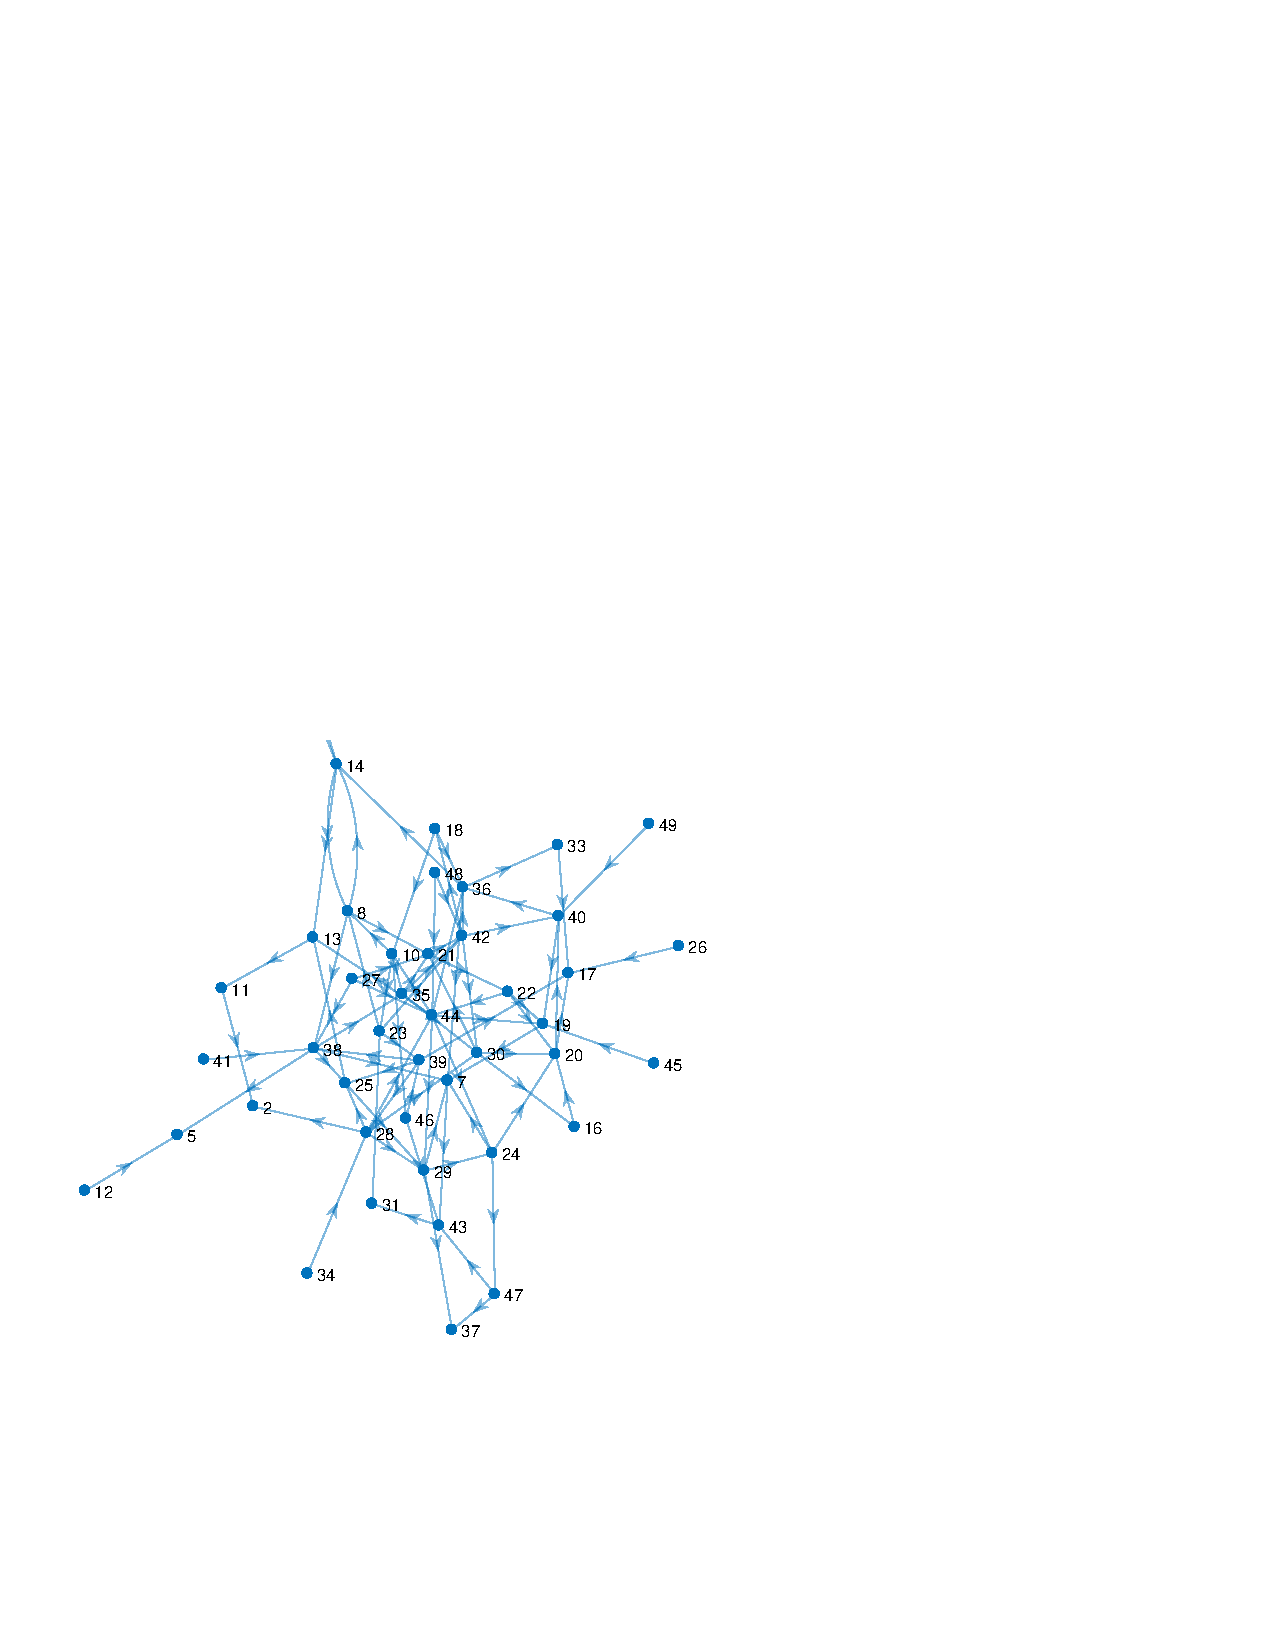
\includegraphics[width=0.8\linewidth]{dag}
\caption{A Directed Acyclic Graph of the Running AUTOSAR Software Application, Runnables = 50, Paths = 35, Activation Patterns shown in Table \ref{tbl_requirements}.}
\label{fig_application}
\end{figure}
\begin{center}
\small
\begin{minipage}{.5\textwidth}%
\centering
\begin{tabular}{@{}p{0.25cm}lll@{}}
\toprule
C& $r_i$ & $(e_{r_im_1}, e_{r_im_2}, e_{r_im_3})$ & $period$\\ \midrule
\multirow{4}{4em}{c1} 
&$r_1$ & (0.030, 0.060, 0.090) & 1\\
&$r_2$ & (0.041, 0.081, 0.122) & 2\\
&$r_3$ & (0.083, 0.167, 0.250)  & 5\\ 
&$r_4$ & (0.310, 0.620, 0.930) & 10 \\[0.3em]
\hline
\multirow{2}{4em}{c2} 
&$r_1$ & (0.310, 0.620, 0.930) & 10\\
&$r_2$ & (0.310, 0.620, 0.930) & 10\\
&$r_3$ & (0.310, 0.620, 0.930)  & 10\\ 
&$r_4$ & (0.310, 0.620, 0.930) & 10 \\[0.3em]
\hline
\multirow{2}{4em}{c3} 
&$r_1$ & (0.310, 0.620, 0.930) & 10\\
&$r_2$ & (0.291, 0.583, 0.874)) & 10\\
&$r_3$ & (0.291, 0.583, 0.874)  & 20\\ 
&$r_4$ & (0.291, 0.583, 0.874) & 20 \\[0.3em]
\hline
\multirow{2}{4em}{c4} 
&$r_1$ & (0.291, 0.583, 0.874) & 20\\
&$r_2$ & (0.291, 0.583, 0.874)) & 10\\
&$r_3$ & (0.291, 0.583, 0.874)  & 20\\ 
&$r_4$ & (0.093, 0.186, 0.279) & 50 \\[0.3em]
\hline
\multirow{2}{4em}{c5} 
&$r_1$ & (0.420, 0.841, 1.261) & 100\\
&$r_2$ & (0.420, 0.841, 1.261)) & 100\\
&$r_3$ & (0.420, 0.841, 1.261)  & 100\\ 
&$r_4$ & (0.420, 0.841, 1.261) & 100 \\[0.3em]
\bottomrule
\end{tabular}
\captionof{table}{Specification of Components.}
\label{tbl_comps_config}
\end{minipage}~
\begin{minipage}{.45\textwidth}
\begin{center}
    \begin{tabular}{@{}lll@{}}
    \toprule
    Activation, $AP$ & Share & Time, ms \\ \midrule
    $\tau_1$ & 50  & 50\\
    $\tau_1\rightarrow\tau_2$ & 20  & 100\\
    $\tau_1\rightarrow\tau_2\rightarrow\tau_3$ & 20  & 200\\
    $\tau_1\rightarrow\tau_2\rightarrow\tau_3\rightarrow\tau_4$ & 10  & 400\\
    \bottomrule
    \end{tabular}
    \captionof{table}{Activation Patters of Cause-effect Chains, their Share and End-to-end Timing Requirements.}
    \label{tbl_requirements}
\end{center}
\begin{center}
    \begin{tabular}{@{}llll@{}}
    \toprule
    M  & $P_{idle}$& $P_{busy}$& $\lambda$ \\ \midrule
    $m_1$ & 50.0& 140.0 &1.0E-3  \\
    $m_2$ & 10.0& 100.0 &1.0E-4  \\
    $m_3$ & 10.0& 140.0 &1 .0E-5 \\ \bottomrule
    \end{tabular}
    \captionof{table}{Computation Nodes Specification.}
    \label{tbl_nodes_specification}
\end{center}
\end{minipage}
\end{center}

In the next subsequent subsections, we propose a metaheuristic approach which is based on Particle Swarm Optimization (PSO) and hybrid PSO. Furthermore, we elaborate the approach using the presented running example.
